\renewcommand{\vec}[1]{\ensuremath{{#1}}}
\newcommand{\Nset}{\ensuremath{\mathbb{N}}\xspace}
\newcommand{\Zset}{\ensuremath{\mathbb{Z}}\xspace}
\newcommand{\Qset}{\ensuremath{\mathbb{Q}}\xspace}
\newcommand{\Cset}{\ensuremath{\mathbb{C}}\xspace}
\newcommand{\Hdivnull}{\ensuremath{Z}}

\fenicschapter{Simulation of transitional flows}
              {Simulation of transitional flows}
              {Simulation of transitional flows}
              {Mikael Mortensen, Kent-Andre Mardal and Hans Petter Langtangen}
              {mortensen}

%------------------------------------------------------------------------------

The purpose of this work is to validate Navier--Stokes (NS) solvers
implemented in FEniCS for unstable, transitional flows. Solvers for
the NS equations have been discussed in Chapter~\ref{chap:kvs-1} for
laminar flows. In this chapter, focus is put more directly on energy
and energy conservation, features of primary importance in turbulence
applications. We emphasize the treatment of the nonlinear convection
term, where various forms (standard, divergence and skew-symmetric) are
implemented and tested for both accuracy and stability. The algorithm
chosen to advance the momentum and pressure in time is a fractional
step approach that is memory efficient, but incurs a splitting error
due to the uncoupling of the velocity and pressure. The significance
of this splitting error is validated through comparison with a more
accurate fully coupled solver that, due to its higher memory cost, is
less suitable for large-scale turbulence applications. The performance
of the solvers is validated with the one-dimensional Burgers' equation,
the Orr--Sommerfeld perturbation in two dimensions and finally the
three-dimensional unstable and transitional Taylor--Green vortex.

\section{Background}

The Navier--Stokes (NS) equations represent a differential form of the
principle of conservation of mass and momentum. They govern both laminar
and turbulent fluid motion in three-dimensional space and time for
incompressible and compressible fluids. There are generally no closed
form analytical solutions to the NS equations and the study of fluid
dynamics thus relies heavily on numerical solutions.

For incompressible Newtonian fluids, the NS equations read
\begin{align}
 \frac{\partial \vec{u}}{\partial t}+\nabla \vec{u} \,  \vec{u}
      &= \nu \nabla^2 \vec{u} -\frac{1}{\rho} \nabla p +\vec{f}, \label{eq:mortensen:NS}
\\
 \nabla \cdot \vec{u} &=0.
 \label{eq:mortensen:cont}
\end{align}
Here $\vec{u}$ is the velocity vector, $\nu = \mu/\rho$
is the kinematic viscosity, where $\rho$ is the density and
$\mu$ is the molecular viscosity, $p$
is the pressure, and volumetric body forces are represented by $\vec{f}$
In the absence of viscosity the principle of energy conservation can
also (in addition to mass and momentum) be directly imposed on the NS
equations. This particular property is especially important for turbulent
flows, since a fundamental feature of turbulence is that kinetic energy
is extracted from the flow system and eventually converted into internal
energy (heat) by the action of viscosity (rate of dissipation). The
largest and most energetic turbulence structures are primarily responsible
for efficient mixing of momentum and other scalar quantities. These
structures are by a series of instability processes broken down to
smaller and smaller spatial scales and eventually dissipated into
heat. The conservation of kinetic energy (in the absence of viscosity)
is thus an important feature of turbulent fluid flows which is formally
consistent with the NS equations. Unfortunately, though, this feature
is not necessarily retained by the numerical scheme used to solve the
discretized NS equations numerically. A numerical method can be both
dissipative and dispersive, recognized for example by the order of the
derivative in the truncation error of Taylor expansions. A numerical
scheme with even order derivatives in truncated terms is dissipative,
whereas odd derivatives lead to dispersion.

The often used terminology Direct Numerical Simulations (DNS) is
understood as the three-dimensional and time dependent numerical
simulations of the NS equations that resolve all all turbulence scales
and that have negligible numerical dissipation (artificial viscosity)
and dispersion. For this reason, DNS are often performed with highly
accurate spectral methods \citep{CanutoHussainiQuarteroniEtAl2007}
in homogeneous flows or higher-order central finite differences or
spectral element methods \citep{Blackburn2009} for more geometrical
flexibility in inhomogeneous flows. The results of carefully executed
DNS have in the fluid mechanics community the same status as carefully
executed experiments. Unfortunately, DNS are very demanding of computer
resources. A good part of the expense is incurred in capturing the
smallest scales of turbulence; that is, the scales that are responsible
for dissipating energy. Yet another complication in non-periodic flows
is to describe inflow and outflow boundary conditions that are consistent
with the NS equations.

The computational cost of DNS can (at the expense of accuracy in
computed statistics) be reduced by capturing only the largest scales
and using a dissipative model in place of the smaller eddies (to
compensate for the loss of accuracy). This method is referred to as
Large Eddy Simulation (LES) and it too requires a three-dimensional and
time-dependent solution. The dissipative model introduces into the NS
equations something that is no longer physically exact. However, to the
extent that the dissipative model does not contaminate the large scales,
LES can provide NS simulations from which statistics may be obtained
with satisfactory accuracy for many purposes. However, the results depend
inherently on the grid, because the grid-independent solution is nothing
but the DNS solution that one in most cases cannot afford. The art of LES
is to find the best possible compromise between efficiency and accuracy.

It should be mentioned that some practitioners of LES use numerical
dissipation to model the unresolved physical dissipation (see the review
of implicit LES given by \citet{Iles}). In this paper, though, we will
only consider numerical schemes with little or no dissipation applicable
for DNS and regular LES.

Turbulent flows and the physical mechanisms responsible for the transition
to turbulence from a laminar flow are not very well understood and
have been researched extensively. At the turn of the 19th century,
Osbourne Reynolds discovered that for cylindrical pipes the transition to
turbulence occurred at a Reynolds number of 2300 ($Re = Uh/\nu$, where
$U$ is the average velocity and $h$ is half the pipe diameter). Later,
with carefully executed experiments in smooth pipes scientists have been
able to increase this number considerably, revealing that velocity is
not really the triggering factor, even though there clearly is a strong
correlation (which follows since as the Reynolds number increases, the
stabilizing viscous damping term becomes comparatively less than the
unstable nonlinear convection term). Another example of transition can
be found in the wakes downstream of bluff bodies placed in an incoming
laminar flow. Here the transition is promoted by the strong shear layer
formed by the recirculation region downstream of the body. In any case,
in order for transition to occur, imposed disturbances triggered by
obstacles, sudden pressure fluctuations, or even a sound waves, must
grow and become unstable and finally chaotic. By introducing systematic
perturbations of the NS equations one can study these phenomena and
watch how they experience resonance and grow or gracefully die. Here,
the numerical scheme will be of utmost importance because a dissipative
scheme will damp (kill) the imposed perturbations.

The most famous early work aimed to study perturbations of the NS
equations was conducted more than 100 years ago by William McFadden
Orr and Arnold Sommerfeld. The epitome of their analytical work
is the celebrated Orr--Sommerfeld equation, which is an eigenvalue
problem describing the linear two-dimensional modes of disturbance to a
viscous parallel shear flow. Although the Orr--Sommerfeld equation only
represents one simplified class of laminar-to-turbulence transition, it
nevertheless constitutes a powerful method to assess numerical schemes
since it provides an analytical transient solution to the NS equations
that remains non-trivial for long integration times. The Orr--Sommerfeld
test case will be further discussed in Section~\ref{sec:mortensen:OS},
but first we need to turn our attention to the NS solvers, the numerical
methods, and their implementation in FEniCS.

\section{Numerical method and energy conservation}
\label{sec:mortensen:Numerical}

In this section we will discuss both the spatial and temporal
discretizations of the Navier--Stokes (NS) equations, and special
attention will be focused on the nonlinear convection term. Furthermore,
since the NS equations represent a system of equations, we will
discuss both a fully coupled method where $\vec{u}$ and $p$ are solved
simultaneously and a fractional step method that solves for the pressure
and velocity in a segregated manner. We also outline the implementation
in FEniCS, and some optimization techniques that can speed up the code
significantly.

\subsection{Convection}
\label{sec:mortensen:Convection}

Let $\Omega \subset \Rset^d$ be an open and bounded region in $\Rset^d$,
where $d$ is the number of spatial dimensions, with smooth boundary
$\Gamma$. The $L^2$ inner product of fields on $\Omega$ is denoted as
\begin{equation}
 \inner{\vec{a}}{\vec{u}} = \int_{\Omega} \vec{a}\cdot \vec{u} \dx,
 \label{eq:mortensen:L2}
\end{equation}
where $\vec{a}$ and $\vec{u}$ are arbitrary vector fields on
$\Omega$. Furthermore, let $L^2$ be the space of square integrable
functions, and we denote the space of divergence-free vector fields
by~$\Hdivnull$.

Let the convective transport of any vector field be written in general form as
$B(\vec{u},\vec{a})$. Here, $\vec{u}$ is the \emph{convecting velocity},
while $\vec{a}$ is the \emph{convected vector field}. Then the standard
convective term,
\begin{equation}
B(\vec{u},\vec{a}) =  \nabla \vec{a} \, \vec{u},
\end{equation}
can be multiplied by the vector $\vec{b}$ and integrated by parts to yield
\begin{equation}
 \inner{ B(\vec{u}, \vec{a})}{\vec{b}}
      = -\inner{\vec{a}}{B(\vec{u},\vec{b})}
        - \inner{B (\vec{a}, \vec{u})}{\vec{b} }
        + \int_{\Gamma} \left(\vec{b} \cdot \vec{a} \right)\left(\vec{u} \cdot \vec{n} \right) \, d\Gamma.
\label{eq:mortensen:Bu1}
\end{equation}
If we for simplicity assume homogeneous Dirichlet boundary conditions
the last term vanishes. Furthermore, if the velocity is divergence-free
($\vec{u}\in \Hdivnull$), the following result can be obtained for the
standard convection form
\begin{equation}
  \inner{ B(\vec{u},\vec{a})}{\vec{b} } = -\inner{ \vec{a}}{ B(\vec{u},\vec{b}) }.
\label{eq:mortensen:Bu2}
\end{equation}
This equation implies that if the standard convective form is adopted
and $\nabla\cdot\vec{u} = 0$, then
\begin{equation}
\inner{ B(\vec{u}, \vec{a})}{ \vec{a} } = 0
\label{eq:mortensen:B0}
\end{equation}
for any choice of $\vec{a}$ (follows by setting $\vec{b}=\vec{a}$ in
\eqref{eq:mortensen:Bu2}). This is an important and necessary result
for conservation of kinetic energy. This observation is perhaps more
transparent if we rewrite the convective term to show that it in fact
represents transport of kinetic energy:
\begin{equation}
\label{eq:mortensen:conv:K}
\left(B(\vec{u}, \vec{u}), \vec{u} \right)
= \int_\Omega (\nabla\vec{u} \, \vec{u})\cdot\vec{u}\dx
= \int_\Omega \vec{u}\cdot\nabla K(\vec{u})\dx
= B(\vec{u}, \vec{u}\cdot\vec{u}),
\end{equation}
where $K(\vec{u})$ is the (specific) kinetic energy of the fluid flow
and is defined as
\begin{equation}
 K(\vec{u})=\frac{1}{2}\, \vec{u}\cdot \vec{u}. \label{eq:mortensen:K}
\end{equation}
The result in \eqref{eq:mortensen:conv:K} means that the integral
contribution from the convection of momentum to the accumulation of
kinetic energy will be zero.

There are several alternative representations of the convective
term. The divergence form
\begin{equation}
B(\vec{u},\vec{a})=\nabla \cdot (\vec{u} \otimes \vec{a})
\end{equation}
follows from the standard format by utilizing the divergence
constraint. The well-known skew-symmetric (or just skew) form is
a combination of the standard and divergence forms
\begin{equation}
 B(\vec{u},\vec{a}) = \frac{1}{2}\left[ \nabla \vec{a} \, \vec{u}\cdot
          + \nabla \cdot (\vec{u} \otimes \vec{a}) \right].
\label{eq:mortensen:skew}
\end{equation}
It can easily be shown, by multiplying \eqref{eq:mortensen:skew} with
$\vec{a}$ and integrating by parts, that the skew-symmetric form of
\eqref{eq:mortensen:skew} ensures that \eqref{eq:mortensen:B0} holds
for any (smooth) velocity field, and not just the divergence-free $\vec{u} \in \Hdivnull$.
This is an important result, because in fractional step (projection)
methods for the NS equations the divergence constraint is not always
fulfilled, at least not for intermediate velocity fields. With the
skew-form it is ensured that this divergence flaw does not propagate
and contaminate the (of primary importance) kinetic energy of the flow.

\subsection{Kinetic energy}
\label{sec:mortensen:kinetic}

A dynamic equation for $K$ can be derived from \eqref{eq:mortensen:NS}
by taking the scalar product of the momentum equation and $\vec{u}$,
and thereafter rearranging using the divergence constraint to arrive at
\begin{equation}
 \frac{\partial K(\vec{u})}{\partial t} + \nabla \cdot [\vec{u}K(\vec{u})]
        = \nu \nabla^2 K(\vec{u}) -\nu \nabla \vec{u} : \nabla \vec{u}
      - \frac{1}{\rho}\nabla \cdot \left(\vec{u}p \right) +\vec{f}\cdot \vec{u}.
 \label{eq:mortensen:K(u)}
\end{equation}
The second term on the right-hand side represents dissipation of kinetic
energy. The role of the remaining terms (neglecting body forces) is
to transport $K(\vec{u})$ within the computational domain. This is
made clear if \eqref{eq:mortensen:K(u)} is integrated over the domain,
neglecting body forces and making use of boundary conditions (all terms
that can be written as divergences will then vanish, because of the
divergence theorem). The well-known identity for the rate of change of
total kinetic energy is obtained (see \citet{SimoArmero1994}):
\begin{equation}
 \frac{\text{d} \Bar{K} }{\text{d} t} = - \nu \int_\Omega \nabla
 \vec{u} : \nabla \vec{u} \dx,
\quad \Bar{K} = \int_{\Omega} K(\vec{u}) \dx .
\end{equation}
Evidently, since $\nu \ge 0$, energy should only decay and not be created
within the domain. For
inviscid flows (Euler equations) $\nu=0$, transport is merely through
the convective term and $\text{d} \Bar{K}/\text{d} t = 0$. This means
that as a consequence of NS equations, energy should be conserved through
convective transport and dissipated only through the action of viscosity.


\subsection{Nature of discretization schemes}
\label{sec:mortensen:dissipative:dispersive}

There are numerous examples of numerical schemes that dissipate
energy. The most familiar in fluid mechanics are probably the stabilizing
upwinding-schemes (favored in many commercial software packages for
their robustness) and streamline diffusion methods in finite element
formulations. In general, numerical schemes that are asymmetric about
the grid point (like upwind schemes) are known to be both dissipative
and dispersive, whereas central (symmetric) schemes are non-dissipative,
yet dispersive. Understanding the fundamental effects of dispersion and
dissipation/diffusion and their relation to numerical discretizations is
a key issue when performing the investigations of the present chapter. We
shall therefore devote some space to illustrate the basic mechanisms,
which can be conveniently done by studying a one-dimensional conservation
equation
\begin{equation}
\frac{D\phi}{dt}
 = \frac{\partial\phi}{\partial t} + v\frac{\partial\phi}{\partial x}
  = 0,
\label{eq:mortensen:phi:pde}
\end{equation}
where $v$ is constant velocity. The initial condition is
\begin{equation}
  \phi(x,0)=f(x).
\end{equation}
Equation~\eqref{eq:mortensen:phi:pde} expresses non-dissipative transport
in the direction of the $x$ axis (if $v>0$), which means that the initial
shape just moves with velocity $v$:
\begin{equation}
 \phi(x,t) = f(x-vt).
\end{equation}
An energy measure $\int_{-\infty}^\infty\phi^2\dx$ remains constant
in time.

We can build an arbitrary shape of $\phi$ as a Fourier series and study
the behavior of one Fourier component.  A complex Fourier mode $\phi
= A\exp{(ik(x - ct))}$ is a solution of \eqref{eq:mortensen:phi:pde}
for an arbitrary amplitude $A$ and frequency $k$, provided $c = v$.
All such components move with constant velocity $v$ and the energy of
each component is constant in time.

Many finite difference schemes for \eqref{eq:mortensen:phi:pde} also
allow Fourier components as solutions. More precisely, we have
\begin{equation}
   \phi_j^n = A\exp{(i(kx - \tilde c t))},
\end{equation}
where $j$ denotes a grid point on the $x$ axis and $n$ denotes the time
level.  The numerical wave velocity $\tilde c \neq v$ is a function of
$k$, $\Delta t$, and $\Delta x$.  When $\tilde c$ is real, but deviates
from the exact value $v$, the Fourier component moves with slightly the
wrong velocity. This dispersion error gives rise to a change of shape
of the solution when we sum all components.  If $\tilde c$ is complex,
the imaginary value will lead to an effective amplitude that either
grows or decreases in time. A growth will make the solution arbitrarily
large for some large $t$, which is unphysical and hence ruled out as an
unstable numerical scheme.  A decrease in amplitude can be tolerated
physically, but the discrete energy $\sum_j |\phi_j^n|^2$ decreases
in time and the wave is said to dissipate.  For this model problem,
the error in $\tilde c$ usually depends on the non-dimensional Courant
number $C\equiv v\Delta t/\Delta x$.

Using a central difference scheme in space and time for
\eqref{eq:mortensen:phi:pde} results in a real $\tilde c$ if $C\leqslant
1$. For $C<1$ the scheme is dispersive, but the discrete energy is
conserved in time.  Choosing $C>1$ gives a complex $\tilde c$ and a
growing discrete Fourier component, which implies $C\leqslant1$ for
numerical stability.

Looking at a forward scheme in time and upwind scheme in space; that
is, two asymmetric differences, the numerical wave velocity $\tilde c$
becomes complex: $\tilde c = \tilde c_r + i\tilde c_i$.  The value
of $c_r$ deviates from the exact velocity $v$, implying dispersion,
while the imaginary value $c_i$ is positive, giving rise to a decreasing
amplitude $A\exp{(-ikc_i n\Delta t)}$ in time.  This is a dissipative
effect of the asymmetric difference(s).  With a decreasing amplitude of
the various Fourier components, the integral of the squared numerical
solution will naturally decrease, and energy is lost.

\subsection{A generic Navier--Stokes discretization}
\label{sec:mortensen:NS-solver}

For the reasons explained above, central difference schemes are usually
favored in the solution of the chaotic and transient velocity fields
governed by the NS equations. Upwind schemes or streamline diffusion,
on the other hand, are often used for Reynolds Averaged Navier--Stokes
(RANS) equations, where the kinetic energy transport is solved for
via a separate PDE and not implied by the computed deterministic mean
velocity field. A Galerkin finite element method, where the basis
functions of the test and trial spaces are the same (modulo boundary
conditions), will produce discrete equations that correspond to central
differencing in space. Therefore, we employ the standard Galerkin method
for spatial discretization. For the temporal discretization we follow
\citet{SimoArmero1994} and describe a family of solvers for the transient
NS equations.

Let $t_n \in \Rset^{+}$ denote a discrete point in time. The velocity
$\vec{u}_{n-1}=\vec{u}(\text{x},t_{n-1})$ is known, and we wish to advance
the solution to $\vec{u}_{n}=\vec{u}(\text{x},t_{n})$.  To this end we
use the following general algorithm
\begin{align}
\label{eq:mortensen:NS_d}
    \frac{\vec{u}_{n}-\vec{u}_{n-1}}{\Delta t}
      &= - B(\tilde{\vec{u}},\Bar{\vec{u}})
          + \nu \nabla^2 \vec{u}_{n-\alpha}
        -\nabla p_{n-1/2} + f_{n-\alpha}
\\
 \label{eq:mortensen:cont_d}
    \nabla \cdot \vec{u}_{n-\alpha} &= 0,
\end{align}
where
\begin{equation}
   \vec{u}_{n-\alpha}=(1-\alpha) \vec{u}_{n} + \alpha \vec{u}_{n-1},
\end{equation}
and $\alpha \in [0, 1]$.  The idea is to discretize all terms at the
time level $n-\alpha$. The nature of the time difference over the interval
$\Delta t = t_n - t_{n-1}$ then depends on $\alpha$. For $\alpha =1/2$
we have a centered scheme
in time, while $\alpha =1$ and $\alpha=0$ are fully explicit and fully
implicit schemes, respectively. Note that at any time the pressure can be
determined from the velocity, and as such it is not directly a function
of time. However, since it appears only on the right-hand side it is
common to compute the pressure at discrete points located at the
midpoint between the time steps where velocity is computed
$t_{n-1/2}, t_{n-3/2}, \ldots$.

The convecting and convected velocity fields
$\tilde{\vec{u}}$ and $\Bar{\vec{u}}$ in the $B$ formula can
be approximated in various ways. The most obvious choice is
$\tilde{\vec{u}}=\Bar{\vec{u}}=\vec{u}_{n-\alpha}$ to be consistent with
the other terms. However, alternative choices may simplify the solution
process. For example, $\tilde{\vec{u}}=\Bar{\vec{u}}=\vec{u}_{n}$ yields
in combination with $\alpha=0$ a consistent nonlinear backward Euler
scheme. An explicit treatment of the convection term is obtained by
$\tilde{\vec{u}} = \Bar{\vec{u}} = \vec{u}_{n-1}$.  A linear implicit
scheme requires that $\vec{u}_{n}$ is present (linearly) in either
$\tilde{\vec{u}}$ or $\Bar{\vec{u}}$, but not in both.

In this work we will make use of one explicit and two implicit
discretizations of the convection term $B$:
\begin{align}
\label{eq:mortensen:EX}
B(\tilde{\vec{u}},\Bar{\vec{u}}) &=
\frac{3}{2}B(\vec{u}_{n-1},\vec{u}_{n-1})-
\frac{1}{2}B(\vec{u}_{n-2},\vec{u}_{n-2}),
\\
\label{eq:mortensen:IM1}
B(\tilde{\vec{u}},\Bar{\vec{u}}) &=
B(\vec{u}_{n-1},\vec{u}_{n-\alpha}),
\\
 \label{eq:mortensen:IM2}
B(\tilde{\vec{u}},\Bar{\vec{u}}) &=
B(\frac{3}{2}\vec{u}_{n-1}-\frac{1}{2}\vec{u}_{n-2},\vec{u}_{n-\alpha}).
\end{align}
The explicit Adams-Bashforth
scheme \eqref{eq:mortensen:EX} is chosen primarily because
of its popularity in the fluid mechanics community. The implicit
schemes use a centered ``Crank--Nicholson'' time discretization
with $\alpha=1/2$ for the convected velocity, in combination with
forward Euler \eqref{eq:mortensen:IM1} and Adams-Bashforth projection
\eqref{eq:mortensen:IM2} for the convecting velocity.
The scheme \eqref{eq:mortensen:IM1} is first-order, whereas the
remaining two are second-order accurate in time (see, for instance,
Figure~3 in \citet{SimoArmero1994}).

Equations \eqref{eq:mortensen:NS_d} and \eqref{eq:mortensen:cont_d}
contain (in three-dimensional space) four unknown fields and four PDEs.
Although the system of equations can be solved in the fully coupled way
formulated in \eqref{eq:mortensen:NS_d} and \eqref{eq:mortensen:cont_d},
it is common to split the system into a set of simpler equations so
that we can compute the velocity and pressure separately.  This class
of approaches is often referred to as fractional step methods.

The fundamental problem in \eqref{eq:mortensen:NS_d} is that the
pressure $p_{n-1/2}$ is unknown. One approximation is to use the
known pressure gradient $\nabla p_{n-3/2}$ from the previous time step
as a first guess. Then, \eqref{eq:mortensen:NS_d} can be solved for
$\vec{u}_n$. Unfortunately, this $\vec{u}_n$ will most likely not also
fulfill \eqref{eq:mortensen:cont_d}. Moreover, there is no obvious way
to advance $p$ to time $t_{n-1/2}$. Still, we may correct the solution
of \eqref{eq:mortensen:NS_d} by using an old pressure. Let us denote
this tentative, or intermediate, solution by $\vec{u}_I$ ($I$ for
intermediate). Its equation is
\begin{equation}
\label{eq:mortensen:NS_FS}
\frac{{\vec{u}}_{I}-\vec{u}_{n-1}}{\Delta t} =
- B_I(\tilde{\vec{u}},\Bar{\vec{u}}) +
\nu \nabla^2 ((1-\alpha) {\vec{u}}_{I} + \alpha \vec{u}_{n-1})
-\nabla p_{n-3/2} + f_{n-\alpha}.
\end{equation}
Note that in the expressions for $B(\tilde{\vec{u}},\Bar{\vec{u}})$ we
replace $\vec{u}_n$ by $\vec{u}_I$, which is why there is a subscript
added to the $B$ term.

We are now interested in correcting for the error $\vec{u}_n-\vec{u}_I$.
Subtracting the exact equation \eqref{eq:mortensen:NS_d} with $\alpha =
0$ from \eqref{eq:mortensen:NS_FS} yields an estimate of the error:
\begin{equation}
\label{eq:mortensen:NS_FS:error}
\frac{{\vec{u}}_{n}-\vec{u}_{I}}{\Delta t} =
-\nabla\Phi + B - B_I + (1-\alpha )\nabla^2(\vec{u}_n-\vec{u}_I),
\end{equation}
where $\Phi = p_{n-1/2} - p_{n-3/2} $ is a pressure correction.  Note that
for an explicit scheme with $\alpha = 1$, only the $-\nabla\Phi$ term
remains on the right-hand side of \eqref{eq:mortensen:NS_FS:error}
since in that case $B = B_I$. Even when $\alpha < 1$ it is common to
drop the terms $B - B_I + (1 - \alpha)\nabla^2(\vec{u}_n-\vec{u}_I)$.
One therefore considers the simplified equation
\begin{equation}
\label{eq:mortensen:NS_FS:error2}
\frac{{\vec{u}}_{n}-\vec{u}_{I}}{\Delta t} =
-\nabla\Phi,
\end{equation}
coupled with the requirement that the new velocity must fulfill:
\begin{equation}
 \label{eq:mortensen:NS_FS:cont} \nabla \cdot \vec{u}_{n} =0.
\end{equation}
We can easily eliminate $\vec{u}_{n}$ from
\eqref{eq:mortensen:NS_FS:error2} and
\eqref{eq:mortensen:NS_FS:cont} by solving for $\vec{u}_{n}$ in the
former and inserting in the latter. This procedure results in a
Poisson equation for $\Phi$:
\begin{equation}
 \label{eq:mortensen:PC} \nabla^2 \Phi = -\frac{1}{\Delta t} \nabla \cdot {\vec{u}}_{I} .
\end{equation}
After solving this equation for $\Phi$, we can finally update the
velocity and pressure from \eqref{eq:mortensen:NS_FS:error2} and the
definition of $\Phi$:
\begin{align}
 \label{eq:mortensen:vel_update} \vec{u}_{n} &= {\vec{u}}_{I} - \Delta t \nabla \Phi, \\
  p_{n-1/2} &= p_{n-3/2} + \Phi .
\label{eq:mortensen:update}
\end{align}
To summarize, the fractional step algorithm involves
solving \eqref{eq:mortensen:NS_FS}, \eqref{eq:mortensen:PC},
\eqref{eq:mortensen:vel_update}, and \eqref{eq:mortensen:update}. The
latter two are trivial, the Poisson equation \eqref{eq:mortensen:PC}
is straightforward, and \eqref{eq:mortensen:NS_FS} is easy to step
forward if $\alpha=1$, otherwise we need to solve a potentially
nonlinear convection-diffusion vector equation.  All of these
equations are simpler than the original coupled problem in
\eqref{eq:mortensen:NS_d}--\eqref{eq:mortensen:cont_d}.

A particular advantage of the fractional step method is that
it opens up the possibility of decoupling the vector equations
\eqref{eq:mortensen:NS_FS} and \eqref{eq:mortensen:vel_update}. The
latter can be updated pointwise, one velocity component at a time. In
a finite element context, however, values of $\nabla\Phi$ at points
where velocity degrees of freedom are defined can be cumbersome
to compute since $\nabla\Phi$ is a discontinuous field. Solving
\eqref{eq:mortensen:vel_update} by projection is then a viable
alternative. Also in this case, we can take advantage of the fact that
\eqref{eq:mortensen:vel_update} are three decoupled scalar equations,
and solve each scalar equation separately. The resulting linear system,
involving a ``mass matrix'', then has the size corresponding to a
scalar partial differential equation and not the triple size
corresponding to the vector formulation in \eqref{eq:mortensen:vel_update}.

With $\alpha =1$ in \eqref{eq:mortensen:NS_FS} the three component
equations decouple so that we can solve one of them at a time. In that
case we get a linear system with a ``mass matrix'' as coefficient
matrix, exactly as when decoupling \eqref{eq:mortensen:vel_update}.
For $\alpha <1$ the convective term may lead to coupling of the component
equations. Treating the convective term explicitly, but allowing
implicitness in the viscosity term implies decoupled component equations
and a possibility to solve a scalar heat or diffusion equation, with
source terms, for each component separately.  The size of coefficient
matrices in the decoupled cases is one third of the size for a coupled
vector equation, leading to much less storage and more efficient
solutions.

A disadvantage of the fractional step method is that even though the
resulting velocity field should be divergence-free due to the pressure
correction~\eqref{eq:mortensen:PC}, the corrected velocity field will
no longer satisfy the discretized momentum equation. This ``splitting
error'' associated with the fractional step method is known to be
first or second order in time depending on whether the pressure is
explicitly included or not included at all in the first velocity step
\citep{GuermondMinevShen2006}. To eliminate the splitting error it is
possible to iterate over the three steps, a practice that is rarely
followed for incompressible flows. A formally superior approach, which
will be explored in this work, is to solve for the velocity and pressure
simultaneously; that is, in a fully coupled manner.  Such a coupled
solver comes at a larger memory cost, which makes it less suitable for
large-scale turbulence applications. However, there is no splitting
error and thus the method can in general take longer time steps and be
particularly useful for validating fractional step solvers.

The convective term contains two velocity fields $\tilde{\vec{u}}$
and $\Bar{\vec{u}}$ that are equivalent in the exact NS-formulation,
but that may differ when discretized. As such, the convective term
$B(\tilde{\vec{u}},\Bar{\vec{u}})$ discussed above can alternatively
be implemented by switching convecting and convected velocities to
$B(\Bar{\vec{u}},\tilde{\vec{u}})$, which in discretized form will
differ from $B(\tilde{\vec{u}},\Bar{\vec{u}})$. Nevertheless, recall
that it is only the first velocity field in $B$ that needs to be
divergence-free for the convection to be energy conservative.
Hence, since the velocity fields
of previous time-steps are (nearly) divergence-free, it is preferable
for fractional step methods to employ an explicit discretization (as
in \eqref{eq:mortensen:EX}--\eqref{eq:mortensen:IM2}) of the first,
convecting velocity. Furthermore, making the convecting velocity implicit
introduces additional coupling between the velocity components, which
makes it less suitable for exploiting enhanced computational efficiency
through solving the component equations one by one.

\paragraph{Implementation in FEniCS}
\label{sec:mortensen:impl_fenics}

The solvers and problems under investigation are implemented in much
the same way as described in Chapter~\ref{chap:kvs-1}, but the naming
convention for the variables is somewhat different. Here we introduce
\emp{u} and \emp{p} for the unknown velocity $\vec{u}_n$ and pressure
$p$ in the variational formulation of the governing equations. The
compound $(\vec{u},p)$ field is named \emp{up} and defined on the
composite space of the velocity and pressure spaces. Such a compound
field is needed in the fully coupled formulation.  Both \emp{u} and
\emp{p} are \emp{TrialFunction} objects, while \emp{up} is of type
\emp{TrialFunctions}.  An appended underscore indicates the most recently
computed approximation to \emp{u}, \emp{p}, and \emp{up}: \emp{u\_},
\emp{p\_}, and \emp{up\_}, all of which are \emp{Function} objects. The
velocities at previous time steps, $\vec{u}_{n-1}$, $\vec{u}_{n-2}$,
$\ldots$, are denoted by \emp{u\_1}, \emp{u\_2}, $\ldots$. These
are \emp{Function} objects. Similarly, \emp{p\_1} represents the old
(corresponding to $p_{n-3/2}$) pressure (\emp{Function}). The quantities
$\tilde{\vec{u}}$ and $\Bar{\vec{u}}$ are named \emp{u\_tilde} and
\emp{u\_bar}, respectively, in the code. Below we only show some key
snippets from the FEniCS implementation.

Given a \emp{Mesh} object \emp{mesh}, a string \emp{mode} describing
the type of formulation of the convective term, and \emp{Constant}
objects \emp{dt} and \emp{nu} for the time step and viscosity, the key
steps in formulating the variational problem for the coupled problem
are as follows:
\begin{python}
V = VectorFunctionSpace(mesh, "Lagrange", 2)  # velocity space
Q = FunctionSpace(mesh, "Lagrange", 1)        # pressure space
VQ = V * Q  # composite space (Taylor-Hood element)
u, p = TrialFunctions(VQ)
v, q = TestFunctions (VQ)
up_  = Function(VQ)
up_1 = Function(VQ)
up_2 = Function(VQ)
u_, p_ = up_.split()
u_1, p_1 = up_1.split()
u_2, p_2 = up_2.split()
u_tilde = 1.5*u_1 - 0.5*u_2
u_bar = 0.5*(u + u_1)

F  = inner(u - u_1, v)*dx + dt*nu*inner(grad(u_bar), grad(v))*dx + \
     dt*conv(u_tilde, u_bar, v, mode)*dx - dt*inner(f, v)*dx - \
     dt*inner(p, div(v))*dx + inner(div(u), q)*dx
a = lhs(F); L = rhs(F)

x_ = up_.vector()  # unknown solution vector (u,p)
dx = Function(VQ)  # correction vector in Newton system
\end{python}
Note that the unknown vector \emp{x\_} in the nonlinear algebraic
equations is just the vector of degrees of freedom in the \emp{up\_}
finite element function so that \emp{up\_} and \emp{x\_} shares
memory. Moreover, \emp{u\_} and \emp{p\_} are parts (views) of
\emp{up\_} and share memory with the latter and \emp{x\_}.  That is,
we can choose between a linear algebra view \emp{x\_} (vector of
degrees of freedom) or a finite element function view \emp{up\_}, or
the velocity part \emp{u\_} or pressure part \emp{p\_} of \emp{up\_}.
In memory there is no duplication of velocity and pressure data.

The three alternative versions of the convective term discussed in
Section~\ref{sec:mortensen:Convection} have be implemented in the method
\emp{conv} as
\begin{python}
def conv(u_tilde, u_bar, v, mode="standard"):
    if (mode == "standard"):
        return inner(grad(u_bar)*u_tilde, v)
    elif (mode == "divergence"):
        return inner(div(outer(u_bar,u_tilde)), v)
    elif (mode == "skew"):
        return 0.5*(inner(grad(u_bar)*u_tilde, v) + \
        inner(div(outer(u_bar, u_tilde)), v))
\end{python}
The fractional step Navier--Stokes solver is somewhat more elaborate
than the fully coupled, since there are more steps involved. The
details of several fractional step solvers are given in
Chapter~\ref{chap:kvs-1}, and thus not repeated here.

\subsection{Speed-up of ``naive'' Navier--Stokes solvers}
\label{sec:mortensen:speed-up}

The previous section presents the straightforward (or naive)
implementation of a coupled vector and scalar equation in FEniCS, using
mixed finite elements.  Examining the structure of the NS equations, one
realizes that many of the terms give rise to similar block matrices in
the coefficient matrix for the complete linear system. The linear system
has size $(n_vd + n_p) \times (n_vd + n_p)$ if $d$ is the number of space
dimensions, $n_v$ is the number of degrees of freedom for a velocity
component field, and $n_p$ is the number of degrees of freedom for the
pressure field.  Several blocks of size $n_v\times n_v$ are identical
since there are three scalar time-derivative terms, giving rise to three
identical mass matrix blocks, and three scalar viscosity (or similarly
convection) terms, giving rise to three Laplacian ``stiffness matrix''
blocks.  Moreover, these blocks are constant in time and do not have to
be reassembled at each time step.

We could gain a potentially significant speed-up by exploiting the
mentioned properties and thereby avoid computing and assembling large
parts of the total coefficient matrix.
This is perhaps not important for smaller two-dimensional problems,
but for larger three-dimensional problems the naive implementation is
much slower than an algorithm exploiting the special structure of the
NS equations.  For CFD practitioners using FEniCS this speed--up is
significant and makes the efficiency of a fairly simple FEniCS-based NS
solver compete with expensive, and much less flexible, state-of-the-art
CFD software.  We shall therefore go through the relevant optimization
steps here in detail.
%%
\begin{enumerate}
 \item Split \emp{F} into accumulation $(\partial \vec{u}/\partial t)$,
   convection $(\nabla \vec{u} \, \vec{u})$, and diffusion terms
   $(\nu\nabla^2 \vec{u})$, and take advantage of the fact that for the total
   coefficient matrix it is only the nonlinear convection term that
   needs to be reassembled at each time step. The matrices for the
   linear, constant-in-time accumulation and diffusion terms can be
   assembled before going into the time loop.

\item For known convecting velocity, the velocity components in
  the momentum equation \eqref{eq:mortensen:NS} are decoupled and
  can as such be solved for in a memory efficient segregated manner,
  treating one component equation at a time with the same (small)
  coefficient matrix. An additional requirement is that some old value
  of $p$ is used, which makes this optimization relevant only for
  velocity steps in a fractional step method.

\item In a fully coupled formulation, we can assemble small
  $n_v\times n_v$ matrices for a term in a component equation and
  insert it into the relevant places in the total coefficient matrix.
  For example, to assemble a convection matrix for one component,
  define a \emp{FunctionSpace} \emp{Vc} for one scalar velocity component 
  identical to the vector space \emp{V.sub(0)}:
\begin{python}
uc = TrialFunction(Vc)
vc = TestFunction(Vc)
Ac = assemble(conv(u_1, uc, vc)*dx)
\end{python}
Here \emp{u\_1} is the \emp{Function} on the space \emp{V} holding the
approximation of the convecting velocity (taken as $\vec{u}_{n-1}$ in
this example).  The matrix \emp{Ac} is of size $n_v\times n_v$ ($n_v$
equals \emp{Vc.dim()}).  The large matrix for the complete velocity
vector field can now be obtained simply by copying this \emp{Ac}
matrix to the three diagonal slots in the $3\times 3$ block matrix
that makes up the whole convection matrix for the velocity vector
field.  At the time of writing, it is for a three-dimensional problem
approximately 20 times faster to assemble this \emp{Ac} than
assembling the $n_vd\times n_vd$ matrix for the complete convection
term $\nabla \vec{u} \, \vec{u}_{n-1}$ by \emp{assemble(conv(u\_1, u,
  v)*dx)}.

\item The right-hand side of the linear system can be reassembled
  at each time step using matrix--vector products and vector additions
  only, a procedure that is described in Chapter~\ref{chap:langtangen}.

\item The sparse coefficient matrix can be compressed by removing
  redundant zeroes. For three-dimensional problems the assembled
  diffusion matrix (using a \emp{VectorFunctionSpace}) contains
  approximately three times as many zeroes as nonzeros, since the
  sparsity pattern of the matrix is determined by the connectivity of
  the degrees of freedom of the finite element fields. The assembled
  zeros slow down Krylov solvers, which rely on fast matrix--vector
  products, as well as preconditioners.

\end{enumerate}
In addition to these steps there are also some simple switches that can
be turned on in the form compiler that optimize the assembly process.

Table~\ref{tab:mortensen:speed-up} summarizes the effect of the
speed-up routines on the CPU-time for the Taylor--Green problem (see
Section~\ref{sec:mortensen:TG}) with $Re=100$ on a \emp{UnitCube} of
size $16^3$ using four time steps and a total integration time
of~$0.5$.  The naive implementations referenced in
Table~\ref{tab:mortensen:speed-up} use one single form for the
Navier--Stokes equations and lhs/rhs to extract forms for the
numerical schemes. This corresponds roughly to the code presented at
the beginning of Section~\ref{sec:mortensen:impl_fenics} for the
coupled solver and similar for the segregated solver. The optimized
versions have been implemented following the steps outlined above. The
two CPU times shown are the total time and the time spent inside the
time integration loop; that is, the total time minus the time it takes
to set up the problem for looping. The two numbers in parenthesis show
the time spent in the Krylov solvers and the assemblers
respectively. Evidently, with the implicit solvers we can for this
problem obtain a speed-up factor of nearly 40 (662/17) for the coupled
solver. Most of this speed--up follows from minimizing the amount of
code that needs to be reassembled every time step and by avoiding a
direct assembly of a large $(n_vd+n_p)\times (n_vd+n_p)$ matrix. As
can be seen, the Krylov solvers are for the optimized solvers
approximately a factor three faster, which is attributed to the
compression of the sparse matrices, which speeds up the matrix--vector
products in the Krylov solvers. It has been verified that the naive
and optimized solvers produce exactly the same results.

\begin{table}
\caption{CPU times (total/inside time loop) for the fully coupled and
  segregated solvers using two different convection schemes in the Taylor
  Green problem. For each solver the first two numbers represent total
  time and time spent in the solver loop. Numbers in parenthesis show
  timings for the solver and assembler respectively.}
\centering
\begin{tabular}{ccccc}
  \toprule
  & \multicolumn{2}{c|}{Fully coupled}   &  \multicolumn{2}{c}{Segregated} \\ [-1ex]
  \midrule
  \raisebox{1.5ex}{Convection}  &  Optimized & Naive & Optimized & Naive \\ [1ex]
  & 46/18 & 170/31 & 45/11   & 134/31 \\ [-1ex]
  \raisebox{1.5ex}{Explicit \ref{eq:mortensen:EX}} & (4.5/3.7) & (11.3/122) & (3.0/2.8) & (8.3/81) \\ [1ex]
  & 45/17 & 688/662  & 44/11 & 498/462 \\ [-1ex]
\raisebox{1.5ex}{Implicit \ref{eq:mortensen:IM2}}& (4.4/3.5) & (10.5/628) & (3.1/2.5) & (8.5/434) \\ [1ex]
\bottomrule
\end{tabular}
\label{tab:mortensen:speed-up}
\end{table}

\section{Numerical investigations}
\label{sec:mortensen:testcases}

In this section, we will look at three popular test cases
for validation of the numerical methods outlined in Section
\ref{sec:mortensen:Numerical}. The simplest and most straightforward
test case is the Burgers' equation, which is widely used in
numerical benchmarks because of its simplicity and resemblance
to the Navier--Stokes equations. The inviscid form of Burgers'
equation will be used to illustrate differences between convective
terms described in Section~\ref{sec:mortensen:Convection}. The second,
more elaborate, test case is the Orr--Sommerfeld eigenvalue problem,
which will be used to evaluate the performance of NS solvers discussed
in Section~\ref{sec:mortensen:NS-solver} for long integration times. The
final test case is the Taylor--Green vortex, which is a three-dimensional
and transient instability problem where an analytical, yet unstable,
initial condition is evolved in a triply periodic domain with no
obstructions.

\subsection{Burgers' equation}
\label{sec:mortensen:burgers}

Burgers' equation reads:
\begin{align}
 \frac{\partial u}{\partial t}+\nabla u \, u
  &= \nu \nabla^2 u, \quad x \in (-1,1), \quad 0<t, \quad u(\pm 1,t)=0,
\\
 u(x,0) &=-\text{sin}(\pi x)+\kappa \xi,
\label{eq:mortensen:burgers}
\end{align}
where $\xi$ is a random number between zero and one and is used to create
a discrete ``white noise'' (uncorrelated) fluctuating velocity field
resembling turbulence, and $\kappa$ is the amplitude of the perturbation.

The variational form of Burgers' equation is obtained by multiplying
\eqref{eq:mortensen:burgers} with test function $v$ and integrating over
the domain, neglecting boundary terms due to the homogeneous Dirichlet boundary
conditions. The resulting variational form involves finding $u_n$ such that
\begin{equation}
 \frac{1}{\Delta t}\inner{ u_{n} - u_{n-1}}{v}
      = - \inner{B(\tilde{u},\Bar{u})}{ v }
          - \nu \inner{ \nabla u_{n-\alpha}}{\nabla v }.
\label{eq:mortensen:burgers_vf}
\end{equation}
We have used Crank--Nicholson-style time discretization ($\alpha=0.5$)
in all our investigations of this case. In one space
dimension the convection terms need some modification from
Section~\ref{sec:mortensen:NS-solver} due to the fact that in one dimension the
velocity is a scalar and the correlation between standard and divergence
forms reads $\nabla u \, u =0.5 \nabla u^2$. To arrive at a skew-symmetric
form the following combination of standard and divergence forms is used
\begin{equation}
 B(\tilde{u},\Bar{u})
    = \frac{1}{3}\left( \tilde{u}\nabla \Bar{u}
      + \nabla \tilde{u} \Bar{u} \right).
\end{equation}
Initialization of the FEniCS \emp{Function u0} can be performed by
subclassing class \emp{Expression} as
\begin{python}
from numpy import sin
from numpy.random import randn
class U0(Expression):
    def eval(self, values, x):
        if(x[0]< -1.+DOLFIN_EPS or x[0]>1.-DOLFIN_EPS):
            # no noise/perturbation at the boundary:
            values[0] = -sin(pi*x[0])
        else:
            values[0] = -sin(pi*x[0])+self.kappa*randn()
u0 = U0(element=V.ufl_element()); u0.kappa = 0.2
u0 = interpolate(u0,V)
\end{python}
The variational problem can be implemented and solved as
\begin{python}
bc = DirichletBC(V, Constant(0), DomainBoundary())

T = 0.25; Nt = 200; k = Constant(T/Nt); t = 0
alfa = Constant(0.5); nu = Constant(0)
u_tilde = u_1 # or u_tilde = 1.5*u_1 - 0.5*u_2 for Adams-Bashforth
u_bar = alfa*(u + u_1)
mode = "standard"  # "skew" or "divergence" (convection term)

F = v*(u - u_1)*dx + k*conv(u_tilde, u_bar, v, mode)*dx + \
    k*nu*u_bar.dx(0)*v.dx(0)*dx
a = lhs(F); L = rhs(F)
u_1 = interpolate(u_, V); u_2 = interpolate(u_, V)
while t < T:
    t = t + dt
    A = assemble(a)
    b = assemble(L)
    bc.apply(A, b)
    solve(A, u_.vector(), b, "gmres", "ilu")
    u_2.assign(u_1); u_1.assign(u_)
\end{python}

Note that the coefficient matrix \emp{A} needs
to be reassembled due to the implicit treatment of
convection. Figure~\ref{fig:mortensen:burgers_KE} shows how the standard,
divergence and skew forms of the convective term perform for the two
implicit solvers. As expected the errors of using the second-order
accurate Adams-Bashforth projection (right) are much smaller than for
the forward Euler method (left). Most noteworthy, though, is the exact
conservation of kinetic energy achieved by the skew form.
As mentioned before, this feature follows simply from the fact that
the assembled matrix \emp{A} is perfectly skew-symmetric -- a feature
that also is retained by the skew form in two- and three-dimensional
cases. Results of using the explicit convection are not shown, since
for the current problem the three convection forms differ only when
treated implicitly.

\begin{figure}
  \centering
  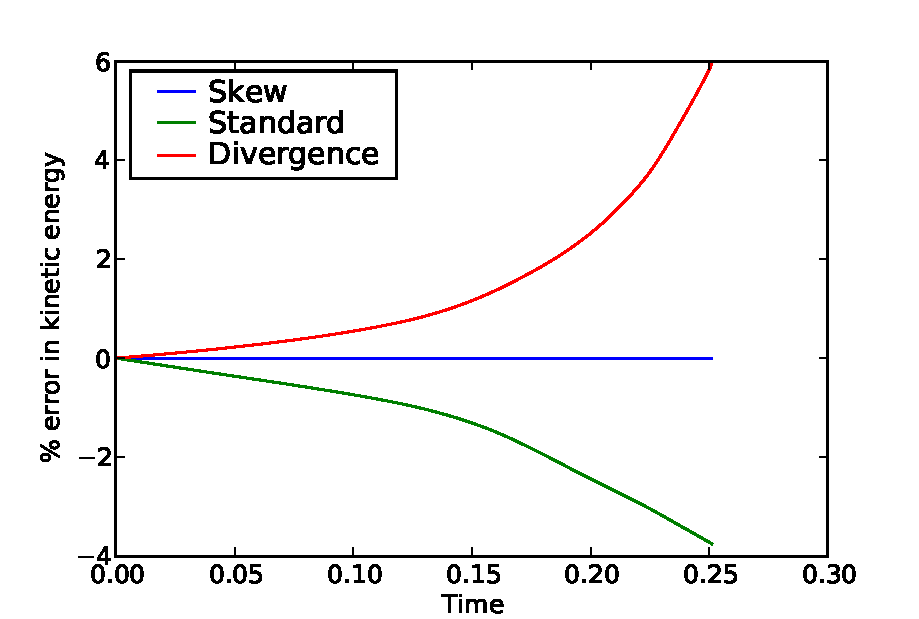
\includegraphics[width=\twofigs]{chapters/mortensen/pdf/Burgers_KE_IM1.pdf}
  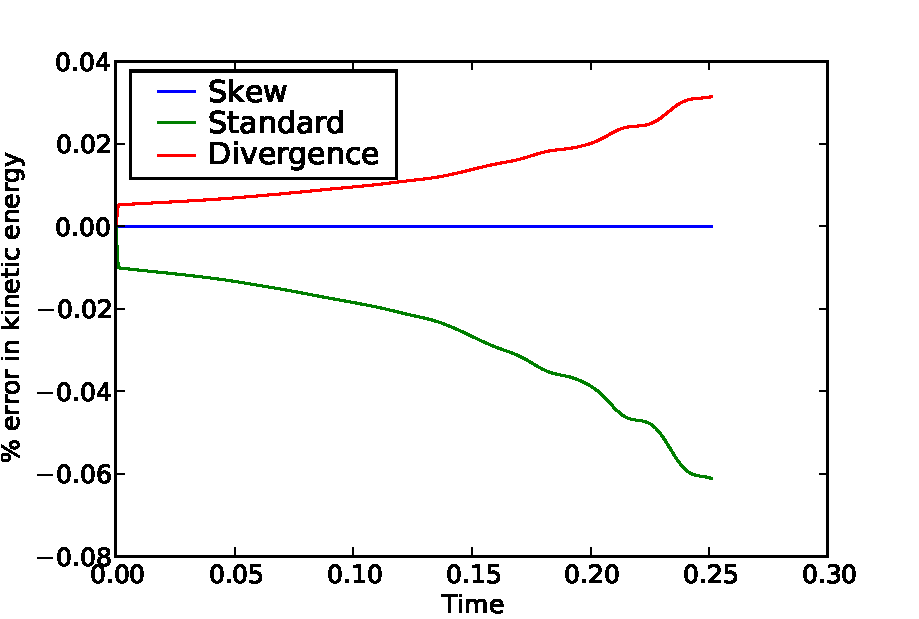
\includegraphics[width=\twofigs]{chapters/mortensen/pdf/Burgers_KE_IM2.pdf}
  \caption{ Accumulation of error in kinetic energy for the inviscid
    Burgers' equation initialized as $u(x,0)=-\text{sin}(\pi x)+0.1
    \xi(x)$. Left and right figures represent the results of using
    \eqref{eq:mortensen:IM1} and \eqref{eq:mortensen:IM2} for
    convection respectively. }
  \label{fig:mortensen:burgers_KE}
\end{figure}

\subsection{Orr--Sommerfeld}
\label{sec:mortensen:OS}

The Orr--Sommerfeld equation (see \citet{Orzag1971}) is derived by
assuming a wave-like disturbance (perturbation) that is proportional to
$\text{exp}(i(\alpha x-\lambda t))$, where $\lambda$ is an eigenvalue
(the complex frequency), $\alpha$
is a prescribed wavenumber (we use $\alpha=1$), $x$ is the streamwise
direction and $t$ is time. The perturbation is applied to the stream
function $\psi(x,y,t)$ such that $\psi=\phi(y) \text{exp}(i(\alpha
x- \lambda t))$, where $\phi$ is the eigenfunction of $\lambda$
and the $y$-direction is normal to $x$ (we consider only two
dimensions). Consequently the velocity perturbations are
\begin{align}
 u'(x,y,t)&=\frac{\partial \psi}{\partial y}=i\alpha \phi \, \text{exp}(i(\alpha x- \lambda t)),
\\
 v'(x,y,t)&=-\frac{\partial \psi}{\partial x}=-\phi' \, \text{exp}(i(\alpha x- \lambda t)).
\end{align}
If we insert this perturbation into the Navier--Stokes equation, an
eigenvalue problem, the Orr--Sommerfeld equation, will appear. The
equation reads
\begin{equation}
 \left( \frac{d^2}{dy^2}-\alpha^2\right)^2\psi
      - \left(\Bar{U}-\lambda \right) \frac{i \alpha}{\nu}
          \left( \frac{d^2}{dy^2}-\alpha^2\right)\psi - \Bar{U}''\psi=0,
 \label{eq:mortensen:OrrS}
\end{equation}
where $\nu$ is the kinematic viscosity and $\Bar{U}(y)$ is the
unperturbed, or basic, velocity.

The Orr--Sommerfeld equation can be solved numerically for any type of
basic flow, but is particularly simple for a channel or Couette flow
where $\Bar{U}$ is known analytically. If the channel spans
$-1\leqslant y \leqslant 1$, then the perturbed velocity in a parallel
channel flow equals
\begin{equation}
\begin{split}
 u(x,y,t)&=1-y^2+\epsilon \,\text{Re}\left(i\alpha \phi \, \text{exp}(i(\alpha x-\lambda t))\right),
\\
 v(x,y,t)&=-\epsilon \, \text{Re}\left(\phi' \, \text{exp}(i(\alpha x-\lambda t))\right),
\end{split}
\label{eq:mortensen:channel}
\end{equation}
where $\epsilon$ is the perturbation amplitude, which needs to be much
smaller than unity.

The Orr--Sommerfeld disturbance evolves very slowly and for $Re=8000$ it
takes approximately $2 \pi/\text{Re}(\lambda)\approx 25$ time units to
travel through the domain. In other words, the NS equations typically need
to be integrated for very long times and the stability of the numerical
time integration scheme thus becomes an important factor. Furthermore,
the Reynolds number may be varied over decades (both the viscous and the
inviscid limits), and a wide range of different solutions may be explored,
as any mode (not just the unstable one) yields a different analytical
solution. Altogether, this makes the Orr--Sommerfeld equation an ideal
test case for NS solvers.

\paragraph{Solution of the Orr--Sommerfeld equation}

The Orr--Sommerfeld eigenvalue problem must be solved with high numerical
accuracy. Here the equations are solved using spectral collocation
with Chebyshev polynomials, as described by \citet{Trefethen2006}. We
consider a channel with Reynolds number $Re=1/\nu=8000$, where
the mean pressure gradient is a constant equal to $2/Re$. Using 80
Chebyshev points the eigenvalues for this problem are plotted in Figure
\ref{fig:mortensen:OS_init}. Note the eigenvalue shown as an open
square ($\lambda =
0.24707506 + 0.00266441 i$), which is the only eigenvalue with a positive
imaginary part. Since the imaginary part is positive, it is evident that
this represents an unstable mode that will grow in time.
Hence one might argue that eventually this disturbance will become
unstable and lead to transition from laminar to turbulent flow.

The Orr--Sommerfeld equation is derived directly from the NS equations
by assuming that the perturbation is small compared to the mean
flow. Hence if the mean flow in a channel is initialized like
\eqref{eq:mortensen:channel}, the instability should grow ``exactly''
like implied by the Orr--Sommerfeld equation
\eqref{eq:mortensen:OrrS}. This has been used to validate NS solvers
by \citet{MalikZangHussaini1984}. The perturbation flow energy is here
used as a measure for the accuracy of the solver:
\begin{equation}
  E(t)= \int_0^{2\pi}\int_{-1}^{1} \left( \left[u-(1-y^2)\right]^2
    + v^2 \right) \dx.
\end{equation}
The exact analytical perturbation energy at any time should be
\begin{equation}
 \frac{E(t)}{E(0)}=\text{exp}(i \text{Imag}(\lambda) t).
\end{equation}
Note, however, that we are looking at the energy of the
\textit{disturbance} only. In other words, we are looking at an
energy transfer drained from the mean field ($\Bar{U}=1-y^2$) into
the perturbation. This is a very different situation from looking at
the total energy of the field, which should be conserved. The energy of
the perturbation increases with time and as such it is no longer evident
that an energy conserving scheme, like the skew form, has any significant
advantage over the not necessarily conservative standard convection form.

\paragraph{Initialization in FEniCS}

The implementation of the Orr--Sommerfeld test-case in FEniCS requires
a two-dimensional computational mesh with associated parameters, like
viscosity, etc. The mesh and some necessary parameters are declared as:
\begin{python}
from dolfin import *
from numpy import arctan
mesh = Rectangle(0.,-1.,2*pi,1.,40, 40)
x = mesh.coordinates()
x[:,1] = arctan(2.*(x[:,1]))/arctan(2.)  # stretch mesh toward wall
Re = 8000.; nu = Constant(1./Re)
f = Constant((2./Re,0.)) # Pressure gradient
\end{python}
where the constant pressure gradient is implemented as a body force
to enable the use of periodic boundary conditions for both velocity
and pressure.

At our disposal we have an Orr--Sommerfeld eigenvalue solver that uses
spectral collocation in $n+1$ Chebyshev points. The details of this
solver is given by \citet{Trefethen2006} and not repeated here, and the
source code can be found in the file \emp{OrrSommerfeld\_eig.py} that
comes with this chapter. For the initialization of DOLFIN \emp{Functions}
with the Orr--Sommerfeld solution, a subclass called \emp{U0} of the
DOLFIN class \emp{Expression} is implemented such that it solves the
eigenvalue problem on creation and overloads the \emp{eval} function
with the equivalence of \eqref{eq:mortensen:channel}. To initialize the
specified initial velocity field we need to create an instance of the
\emp{U0} class and interpolate in the appropriate function space:
\emp{V} for fractional step and \emp{VQ} for the coupled solver. The
procedure for the fractional step solver is:
\begin{python}
# Using 80 Chebyshev points and Reynolds number of 8000:
u = U0(element=V.ufl_element(), defaults={"Re":8000., "N":80})
u_ = interpolate(u, V)
p_ = Constant(0.)
\end{python}
For the coupled solver, \emp{VQ} is used in place of \emp{V}
and the pressure needs to be set in \emp{U0}. The Orr--Sommerfeld
perturbation leads to a non-trivial solution that evolves in
time. The initial perturbed velocity field is illustrated on the left
of Figure~\ref{fig:mortensen:OS_init}.

\begin{figure}
\bwfig
  \centering
  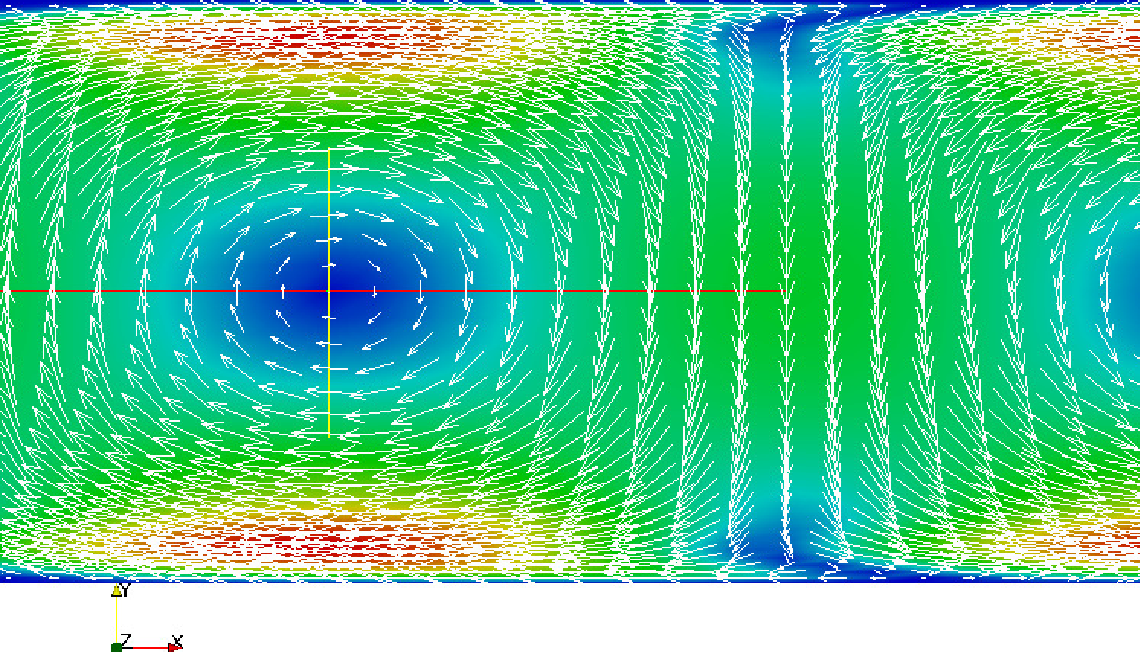
\includegraphics[width=\twofigs]{chapters/mortensen/pdf/OS_init.pdf}
  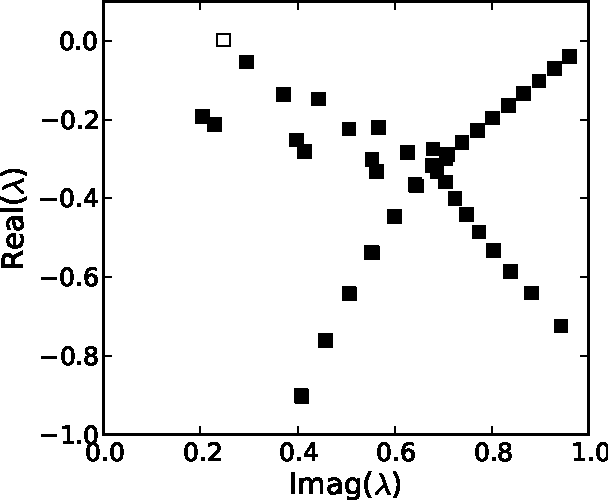
\includegraphics[width=\twofigs]{chapters/mortensen/pdf/OrrS_eigvals.pdf}
  \caption{The left figure shows a snapshot of the initial perturbed velocity
    field. The figure on the right shows the eigenvalues for the Orr Sommerfeld equation
    at $Re=8000$. Note the open square, which is the only eigenvalue
    with a positive imaginary part. This represents an unstable mode.}
  \label{fig:mortensen:OS_init}
\end{figure}

\paragraph{Results}

In this section we consider first the transient behavior of the
Navier--Stokes solver using all three forms of convection discretization
(standard, divergence and skew). The spatial discretization is kept
well resolved with a Rectangle mesh class using $N=48$ and the CFL number
based on the mean velocity ($\Bar{U}=1$~ms$^{-1}$) is varied from 0.5
to 0.025. Figure \ref{fig:mortensen:OS_init_cfl} shows the accumulated
error in the perturbation flow energy computed as
\begin{equation}
 \text{Error} = \sum_{k=0}^N \frac{|E(t_k)-\text{exp}(i \text{Imag}(\lambda) t_k)|}{N}.
 \label{eq:mortensen:error}
\end{equation}
%%
\begin{figure}
  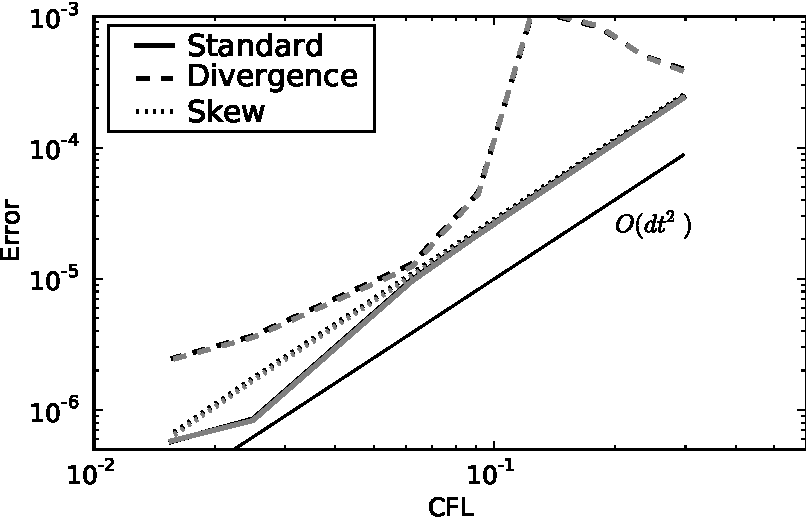
\includegraphics[width=\twofigs]{chapters/mortensen/pdf/OS_init_cfl_1.pdf}
  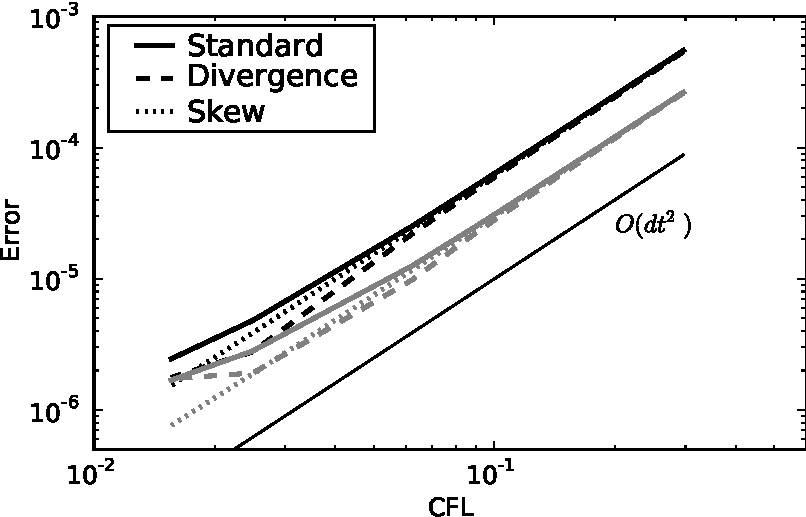
\includegraphics[width=\twofigs]{chapters/mortensen/pdf/OS_init_cfl_0.pdf}
  \caption{Accumulated error \eqref{eq:mortensen:error} vs CFL number
    for an integration time of 0.5 for standard, divergence and skew
    forms, here represented with solid, dashed and dotted lines
    respectively. The fully coupled and fractional step solvers are
    represented with gray and black lines, respectively. All results
    for a mesh size of $N=48$. The figures on left and right
    use explicit \eqref{eq:mortensen:EX} and implicit \eqref{eq:mortensen:IM2}
    convection respectively. Note that for the left figure the black and gray curves
    are practically identical (the error in the fully coupled solver is
    approximately 2\% less throughout). }
  \label{fig:mortensen:OS_init_cfl}
\end{figure}
\begin{figure}
  \centering
  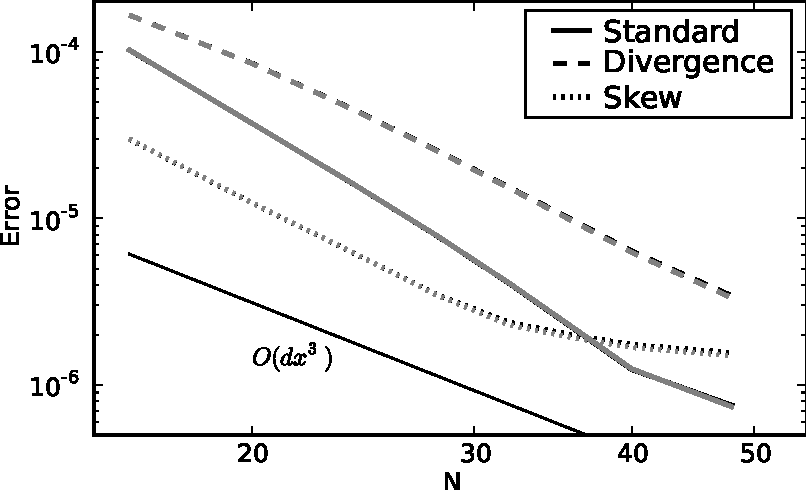
\includegraphics[width=\twofigs]{chapters/mortensen/pdf/OS_init_dx_1.pdf}
  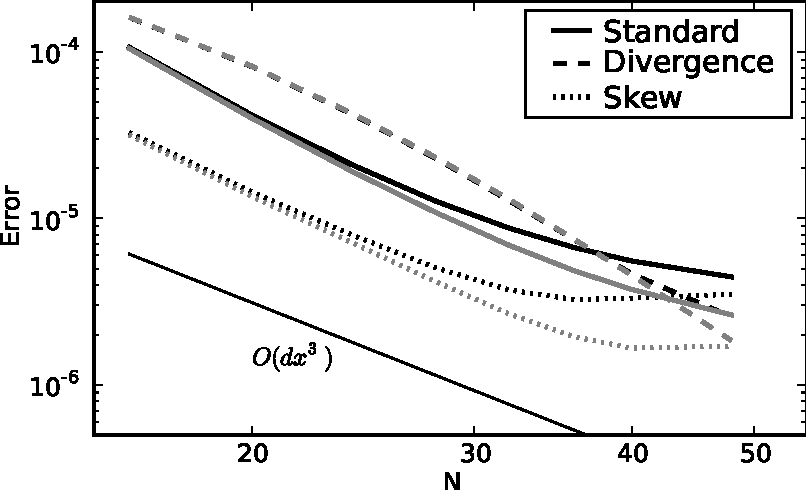
\includegraphics[width=\twofigs]{chapters/mortensen/pdf/OS_init_dx_0.pdf}
%
 \caption{Accumulated error \eqref{eq:mortensen:error} vs mesh size
   for an integration time of 0.5. Standard, divergence and skew forms
   of convection are here represented with solid, dashed and dotted
   lines respectively. The fully coupled and fractional step solvers
   are represented with gray and black lines, respectively. For all
   results the time step used is 0.005. The figures on left and right
   use explicit \eqref{eq:mortensen:EX} and implicit \eqref{eq:mortensen:IM2}
   convection respectively. Note that for the figure on the left the black and
   gray curves are practically identical (the error in the fully
   coupled solver is approximately 2\% less throughout). }
\label{fig:mortensen:OS_init_dx}
\end{figure}
Note that the integration time is kept quite low (from 0 to 0.5), in an
effort to maintain stability for all schemes. However, using explicit
convection the divergence form is still unstable for the highest
CFL numbers. From Figure~\ref{fig:mortensen:OS_init_cfl} we observe
second-order accuracy in time and register that the accuracies of explicit
and implicit methods for convection are similar. With
implicit convection the superior accuracy of the coupled scheme versus the
fractional step solver is evident, and the coupled scheme achieves the same
accuracy with twice the CFL number, which is attributable to
the splitting error. Using explicit convection, there is hardly any
difference between fractional step and coupled solvers (the difference
in the error is approximately 2\% in the favor of the coupled solver
throughout), indicating that the divergence of the intermediate velocity
is small. Another interesting feature is that for explicit convection
the standard form seems to be most accurate followed by the skew and
divergence forms, whereas the opposite behavior is observed for
the implicit solver.

To investigate the spatial discretization with P2/P1 elements, we
keep the time step constant and small at 0.005 and vary the mesh size
from 16 to 48 in the \emp{Rectangle} class. The accumulated error is
shown in Figure~\ref{fig:mortensen:OS_init_dx}, where we observe the
third-order accuracy that is expected for Taylor-Hood elements. Again,
the coupled solver performs better than the fractional step solver
with implicit convection, whereas the solvers are practically identical
with explicit convection. The larger splitting errors obtained with the
fractional step solver using implicit treatment of convection (in both
Figs.~\ref{fig:mortensen:OS_init_cfl} and \ref{fig:mortensen:OS_init_dx})
can be understood by thinking of the fractional step solver as an operator
splitting routine where the implicit diffusion and convection terms are
neglected in the second pressure step. If the convection term is treated
explicitly then the treatment is exact (since the old velocity is used in the
term anyway). Hence, there is only an inconsistency for the diffusion
that is being computed in the first step with an intermediate and not
the end-of-step velocity field. With implicit convection as well, both
diffusion and convection terms are computed with the intermediate (not
divergence-free) velocity field and the inconsistency with the superior
fully coupled scheme becomes more profound.

To validate the more interesting (from a turbulence instability point of
view) long-term performance of the solvers,
we integrate the equations as long as it takes for the perturbation to
travel through the domain two times (end time $\approx$ 50). One single
well-resolved mesh is used ($N = 40$ in the \emp{Rectangle} class) and
the CFL number is set to 0.05 or 0.1 to limit the temporal discretization
errors. Figure \ref{fig:mortensen:OS_long_time} shows the evolution of
the perturbation energy using both the fully coupled and fractional step
solvers with the second-order implicit convection \eqref{eq:mortensen:IM2}
and the second-order explicit scheme \eqref{eq:mortensen:EX}. Evidently,
the standard form of convection is more stable than the divergence (most
unstable) and skew forms for long integration times. The divergence and
skew forms cannot capture the true evolution of the instability and the
solution quickly blows up into a chaotic two-dimensional ``turbulence''
field. The standard form seems to capture the instability with ease and
evolves more or less according to the true solution of the eigenvalue
problem. There are only minor differences between the fractional step
and the fully coupled solver, which is not unexpected since we are
using a very short time step and the error in fractional step splitting
(the only difference between the two methods) is thus minimized. By
increasing the CFL number it can be shown that the fully coupled solver
remains accurate for longer time steps. Note that the total kinetic
energy remains more or less constant for all the simulations shown
in Figure~\ref{fig:mortensen:OS_long_time}, even for the divergence
and skew forms. Hence, the ability of the skew form to maintain total
kinetic energy does not seem to be all that important when we are really
interested in solving instability problems, where the most important
physical process is that energy changes form (from the mean flow to the
perturbation). Also plotted with circles in Figure~\ref{fig:mortensen:OS_long_time}
is the result of using the same number of degrees of freedom
and time step with a standard cell-vertex based finite volume solver.
The finite volume solver is discretized in a similar manner as our
FEniCS solvers with implicit convection \eqref{eq:mortensen:IM2}
using Adams-Bashforth projection and Crank--Nicholson diffusion. The
integration method is fractional step, which is here slightly dissipative
due to the collocated nature of the pressure and velocity. The implicit
higher-order (P2/P1) FEniCS solvers are evidently much better at
capturing this instability than the lower-order finite volume method,
which is not surprising. The difficulties that low-order finite
difference methods face when trying to capture the Orr--Sommerfeld
instability have been reported by \citet{MalikZangHussaini1984} and
\citet{CanutoHussainiQuarteroniEtAl2007}.

\begin{figure}
  \centering
  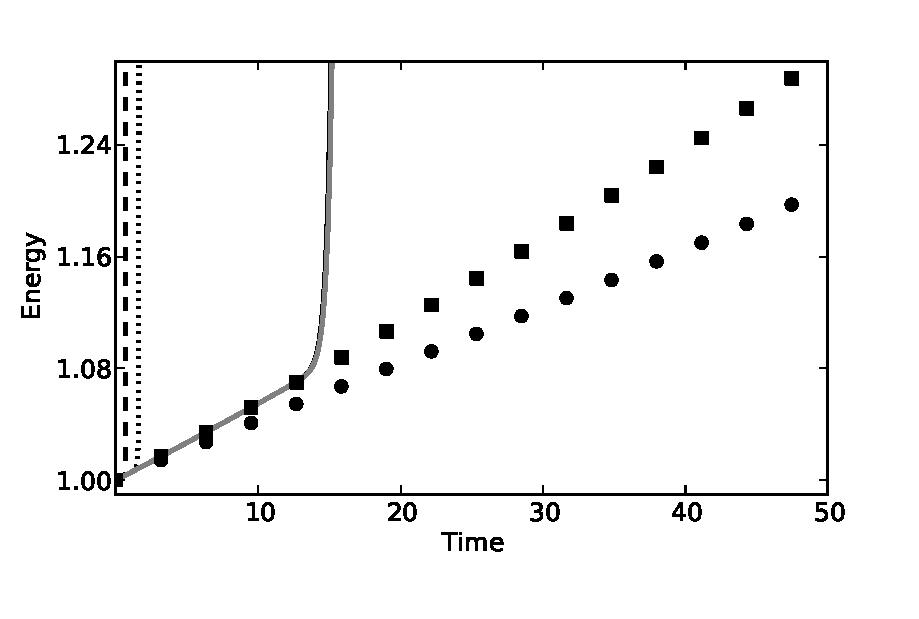
\includegraphics[width=\twofigs]{chapters/mortensen/pdf/OS_energy_cfl_0_1_model_1.pdf}
  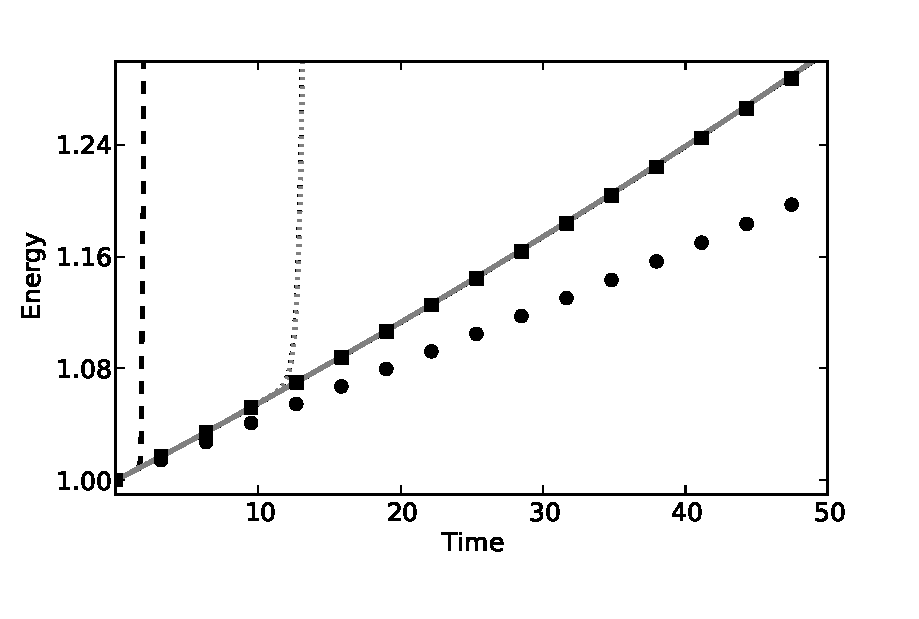
\includegraphics[width=\twofigs]{chapters/mortensen/pdf/OS_energy_cfl_0_1_model_0.pdf} \\
  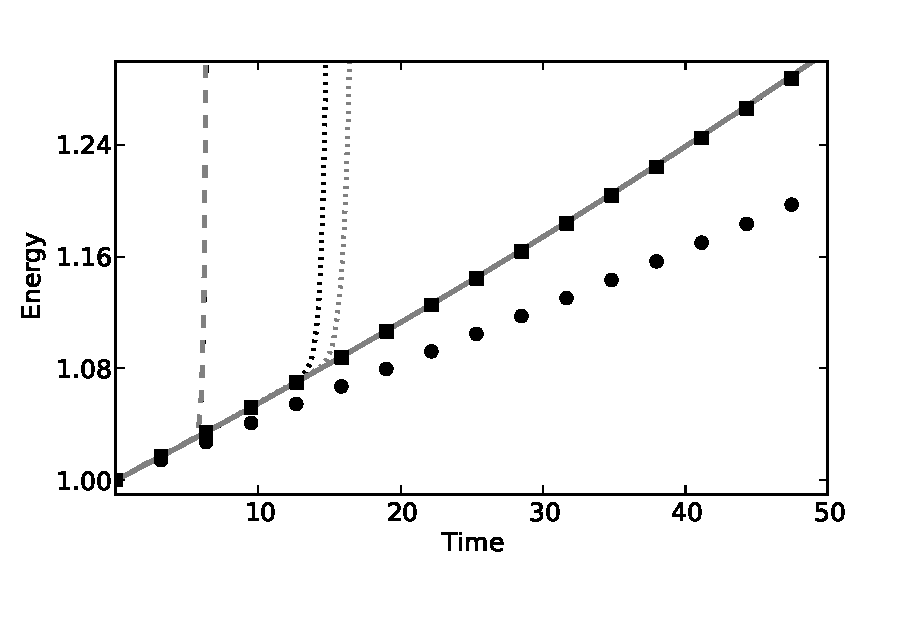
\includegraphics[width=\twofigs]{chapters/mortensen/pdf/OS_energy_cfl_0_05_model_1.pdf}
  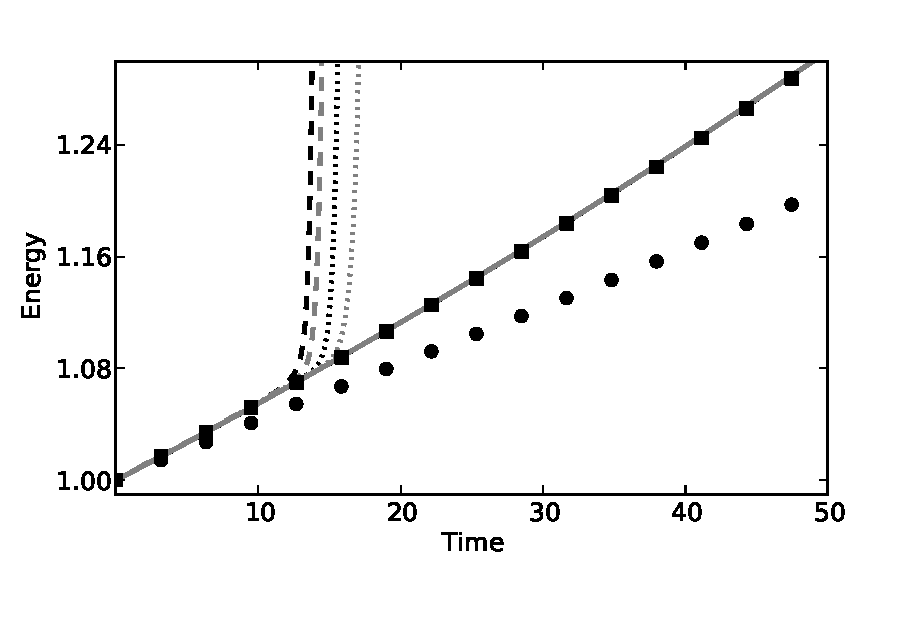
\includegraphics[width=\twofigs]{chapters/mortensen/pdf/OS_energy_cfl_0_05_model_0.pdf}
  \caption{Temporal evolution of the perturbation energy. The gray and
    black lines correspond to the fully coupled and fractional step
    solvers respectively and the solid, dashed and dotted lines
    correspond to the standard, divergence and skew forms of the
    convection respectively. The symbolic dots represent the solution
    from a low-order finite volume solver and the squares represent the
    true solution. The left and right figures on the top row use explicit convection
    as in~\eqref{eq:mortensen:EX}, with CFL of 0.1 and 0.05 respectively.
    The left and right figures on the lower row use implicit convection \eqref{eq:mortensen:IM2} and CFL =
    0.1 and 0.05 respectively. Note that for explicit convection and the standard
    implicit form the gray and black curves are practically
    identical. }
\label{fig:mortensen:OS_long_time}
\end{figure}


\subsection{Taylor--Green vortex}
\label{sec:mortensen:TG}

Finally, we consider a real transition to turbulence problem. The
Taylor--Green vortex is characterized by an initialization based on
an asymptotic expansion in time in a triply periodic domain spanning
$[-\pi,\pi]$ in all three directions. The initial condition is:
\begin{align}
 u(x,y,t)&=\sin(x)\cos(y)\cos(z),
\\
 v(x,y,t)&=-\cos(x)\sin(y)\cos(z),
\\
 w(x,y,t)&=0.
\end{align}
The asymptotic expansion is known to diverge for $t \ge 3$, as the flow
turns turbulent.

Due to the large memory requirements of this three-dimensional
problem, we consider here only the fractional step solver. For validation
we use the total kinetic energy and the total energy dissipation rate,
computed respectively as
\begin{align}
 q &= \frac{1}{2} \int_{\Omega} \vec{u} \cdot \vec{u}, \label{eq:mortensen:q}
\\
 \varepsilon &= \nu \int_{\Omega} \nabla \vec{u}: \nabla \vec{u}. \label{eq:mortensen:diss}
\end{align}
The average rate of dissipation is, as already mentioned, the single
most important measure of a turbulent flow. It is implemented in FEniCS as
\begin{python}
assemble(nu*inner(grad(u_),grad(u_))*dx)/(2*pi)**3.
\end{python}

Since the Taylor--Green vortex is (eventually) a turbulent flow there
is no analytical solution that can be used to compare our results
with. Hence, for validation the Taylor--Green vortex has also been
simulated with Semtex~\citep{Blackburn2009}, which is a well-tested
open source spectral element Navier--Stokes solver that runs in
parallel. Semtex uses quadrilateral spectral elements with standard
nodal Gauss--Lobatto--Legendre basis functions and Fourier expansions
in one homogeneous direction. To validate the Taylor--Green case we
use Semtex with $30 \times 30$ homogeneous elements of order six in both $x$
and $y$-directions and 144 planes in the $z$-direction that is solved
using Fourier expansions. The time step used for the validation simulations
is set to 0.005.

Figure~\ref{fig:mortensen:dissipation} shows the error in average
rate of dissipation and kinetic energy computed using $Re=100$ and
a \emp{UnitCube} domain with $16^3$, $24^3$ and $32^3$ bricks (each
being divided into six tetrahedra). The CFL number used is 0.05, which
practically eliminates temporal errors. With this small time step it is
nearly impossible to distinguish between the results of using explicit
\eqref{eq:mortensen:EX} or implicit \eqref{eq:mortensen:IM2} convection
and thus only the latter is shown.
\begin{figure}
  \centering
  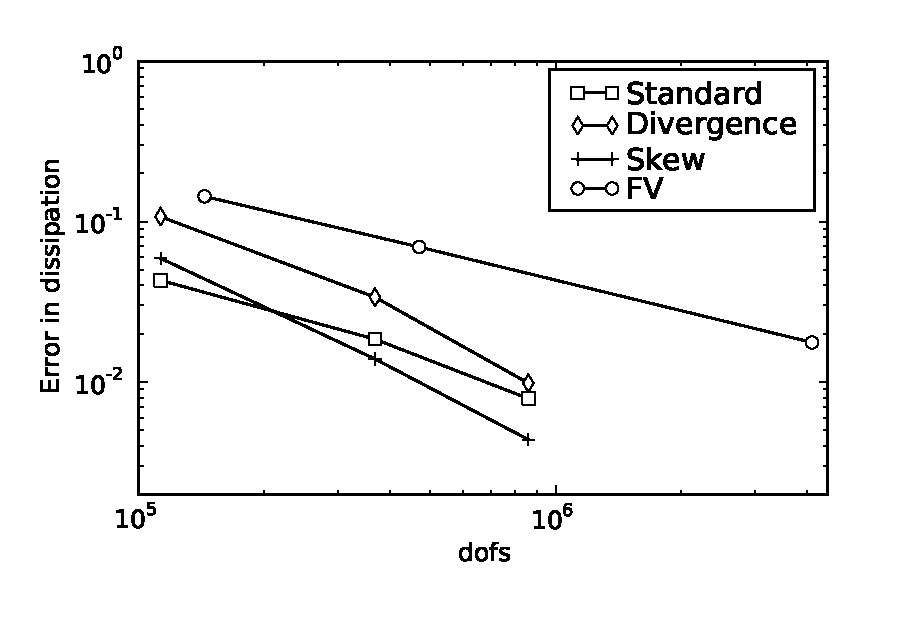
\includegraphics[width=\twofigs]{chapters/mortensen/pdf/TG_disserror_model_0_cfl_0_05_Re_100_dofs.pdf}
  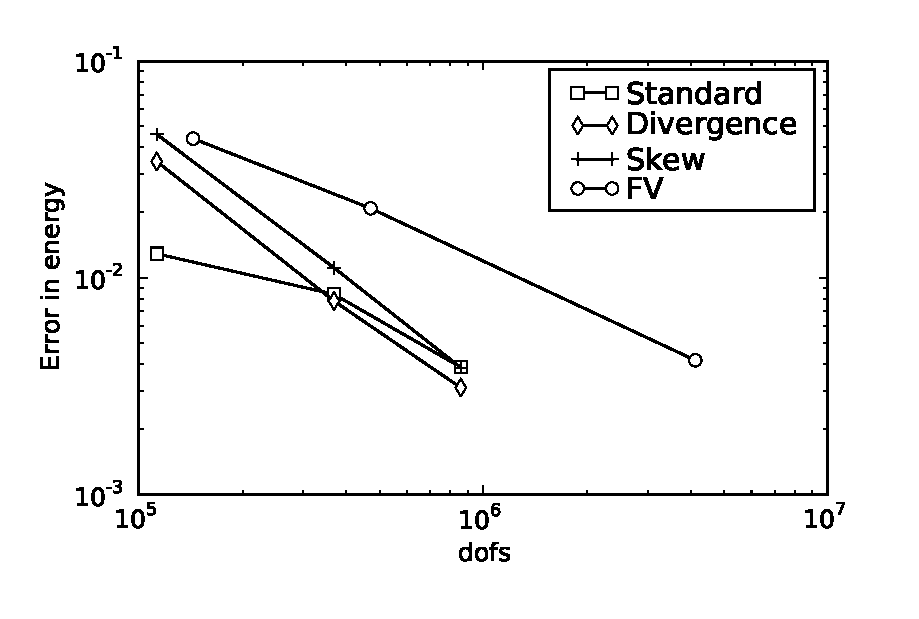
\includegraphics[width=\twofigs]{chapters/mortensen/pdf/TG_energyerror_model_0_cfl_0_05_Re_100_dofs.pdf}
  \caption{Relative errors in dissipation rate \eqref{eq:mortensen:diss} is
    shown in the left figure and the energy \eqref{eq:mortensen:q} in the right. The
    results are displayed for implicit convection
    \eqref{eq:mortensen:IM2}, and the squares, diamonds and pluses
    are used to represent standard, divergence and skew forms
    respectively. The open circles represent the solution obtained
    with a low-order finite volume code and the reference solution
    upon which the error is based is computed with
    Semtex~\citep{Blackburn2009}. }
  \label{fig:mortensen:dissipation}
\end{figure}
The conclusion that can be drawn from
Figure~\ref{fig:mortensen:dissipation} is that the standard convection
form performs less satisfactory than both the skew and divergence
forms. The skew form is best at capturing the average dissipation rate,
whereas the divergence form does a slightly better job at capturing the
total energy. Furthermore, the additional accuracy of
higher-order elements is evidently superior to a low-order finite volume
solver, both for the energy and the dissipation rate.

\section{Conclusions}

In this work we have validated FEniCS-based Navier--Stokes solvers
aimed at applications involving turbulence and instabilities with
transition to turbulence. Such solvers are of particular relevance
to blood flow in the vicinity of aneurysms.  Our focus has been on
flow energy and energy conservation, features of great importance for
turbulent flows. Discretizations of the nonlinear convection term have
been considered both with standard, divergence and skew-symmetric forms
- forms familiar from the vast literature on NS solvers. The numerical
discretizations and solvers have been validated using Burgers' equation,
the Orr--Sommerfeld perturbation to a plane channel flow in two dimensions
and the three-dimensional unstable and transitional Taylor--Green
vortex. We have briefly described the details of our NS solvers and
outlined some optimizations that in our experience provide a speed-up
of more than an order of magnitude compared to straightforward (naive)
FEniCS implementation.

Two fundamentally different approaches to solving the NS equation have
been tested: the fractional step method, which uncouples the velocity from
the pressure, and a fully coupled solver. The fractional step method is
generally favored by most CFD practitioners due to memory efficiency,
even though it introduces a splitting error through uncoupling the
velocity field from the pressure. The coupled solver naturally requires
more memory, but on the other hand there is no splitting error as it
simultaneously satisfies both the discretized momentum equation and
divergence constraint.  The splitting error introduced by the fractional
step solver has been found here with the Orr--Sommerfeld test case to
be small when convection is treated explicitly and enhanced when the
convection term is treated semi-implicitly. With semi-implicit convection
the fractional step method requires the CFL number to be half that of
the coupled solver to achieve the same accuracy. The problem met by
implicit discretizations of the fractional step method
is here attributed to the fact that implicit terms are computed from the
(not necessarily divergence-free) intermediate velocity, as opposed to
the divergence-free, end-of-step, velocity field.
For the long integration times often associated with turbulence
applications, though, we find that the implicit form remains stable and
accurate where the explicit form cannot maintain sufficient stability.

For the Orr--Sommerfeld test case the standard form of convection seems
to be the only form that remains stable for long integration times, even
though the other forms are more accurate initially. For the Taylor--Green
test-case the standard form is found to be less accurate than both the
divergence and skew forms. Further studies with higher Reynolds numbers
are required to more thoroughly validate the stability of NS solvers in
the fully turbulent regime.
